\setcounter{chapter}{2}

\chapter{Coalition Formation for Autonomous Web Services}\label{sec:coalitionformationws}

In this chapter, we present our coalition model of agent-based web
services within communities\cite{SCC2013efficient}. We start by describing the general
architecture and considered parameters for web services.
Thereafter, problem modeling and formulation will be introduced in
terms of task distribution and community revenue. Web service
cooperative games in different settings will follow along with
some simulation results.

\section{Preliminaries}\label{s:preliminaries}

In this section, we discuss the parameters and preliminary
concepts that we use in the rest of the proposal.

\subsection{Architecture}

Our system consists of three main types of entities working
together:

\emph{1) Web services} are rational entities that aim to maximize
their utilities by providing high quality services to end users.
They aim to maximize their individual income by receiving enough
requests from end users. In order to increase their revenue, web
services seek for more tasks if they have the capacity and
throughput to do so. Web services can join communities to have
better efficiency by collaborating with others, to have access to
higher market share, and to have opportunity of receiving a bigger
task pool from end users. Throughout this proposal, in our
equations, we refer to web services as $ws$ and to the set of web
services hosted by a given community as $C$. To simplify the
notation, sometimes we simply write $ws$ instead of $ws \in C$ to
go through the elements $ws$ of the set $C$.

\emph{2) Master Web Services} or the community coordinators, are representatives of the
communities of web services and responsible for their management.
Communities receive requests from users and aim to host a healthy
set of web services to perform the required tasks. They seek to
maximize user satisfaction by having tasks accomplished according
to the desired QoS. In fact, higher user satisfaction will bring
more user requests and increase the market share and revenue of
the community.

\emph{3) Users} generate requests and try to find the best
available services. User satisfaction is abstracted as function of
quantity and quality of tasks accomplished by a given service.
Higher user satisfaction leads to higher trust of the community by users hence directing more requests towards that service provider.

\subsection{Web Service Parameters}\label{ws_parameters}

Web services come with different quality of service parameters.
These parameters with a short description are listed in Table
\ref{qosws}.

\begin{table}[!t]
\centering
\caption{List of web service QoS parameters.}
\begin{tabular}{|c|c||c|c|}
\hline
\textbf{Parameter} & \textbf{Definition} \\
\hline\hline
$Availability$ & Probability of being available during \\
&a time frame \\
$Reliability$ & Probability of successfully handling \\
&requests during a timeframe\\
$Successability$ & Rate of successfully handled requests \\
$Throughput$ & Average rate of handling requests \\
$Latency$ & The average latency of services\\
$Capacity$ & Amount of resources available\\
$Cost$ & Mean service fee \\
$Regulatory$ & Compliance with standards, law and rules\\
$Security$ & Quality of confidentiality \\
&and non-repudiation\\
\hline
\end{tabular}
\label{qosws}
\end{table}


We adopted a real world dataset \cite{DBLP:conf/smc/Al-MasriM09a}
which has aggregated and normalized each of these parameters to a
real value between 0 and 1. Since requests are not shared among
web services and are distributed among all of them inside a
community, each one of them comes with a given QoS denoted by
$(QoS_{ws})$. We assume that $(QoS_{ws})$ is obtained by a certain
aggregation function of the parameters considered in Table
\ref{qosws}. We use this quality output later in evaluating the
community \emph{worth} or \emph{payoff} function.

\subsection{Web Service Communities}\label{webservice-communities}

Figure 3 represents our revised architecture of web service
communities where tasks are to be distributed among the members
that are interested in forming stable coalitions. As discussed in
Chapter 2, communities are essentially virtual platforms
aggregating web services having similar and complementary
functionalities and communicate with other entities such as UDDI
registries and users using particular protocols. Web services join
communities to increase their utility by having larger market
share and task pool. Community coordinators or master web services
are responsible for community development, managing membership
requests from web services and distributing user tasks among the
community members. Community coordinators try to attract quality
web services and keep the community as stable and productive as
possible to gain better reputation and user satisfaction, which
results in having higher revenue.

\begin{figure*}[!t]
\centerline{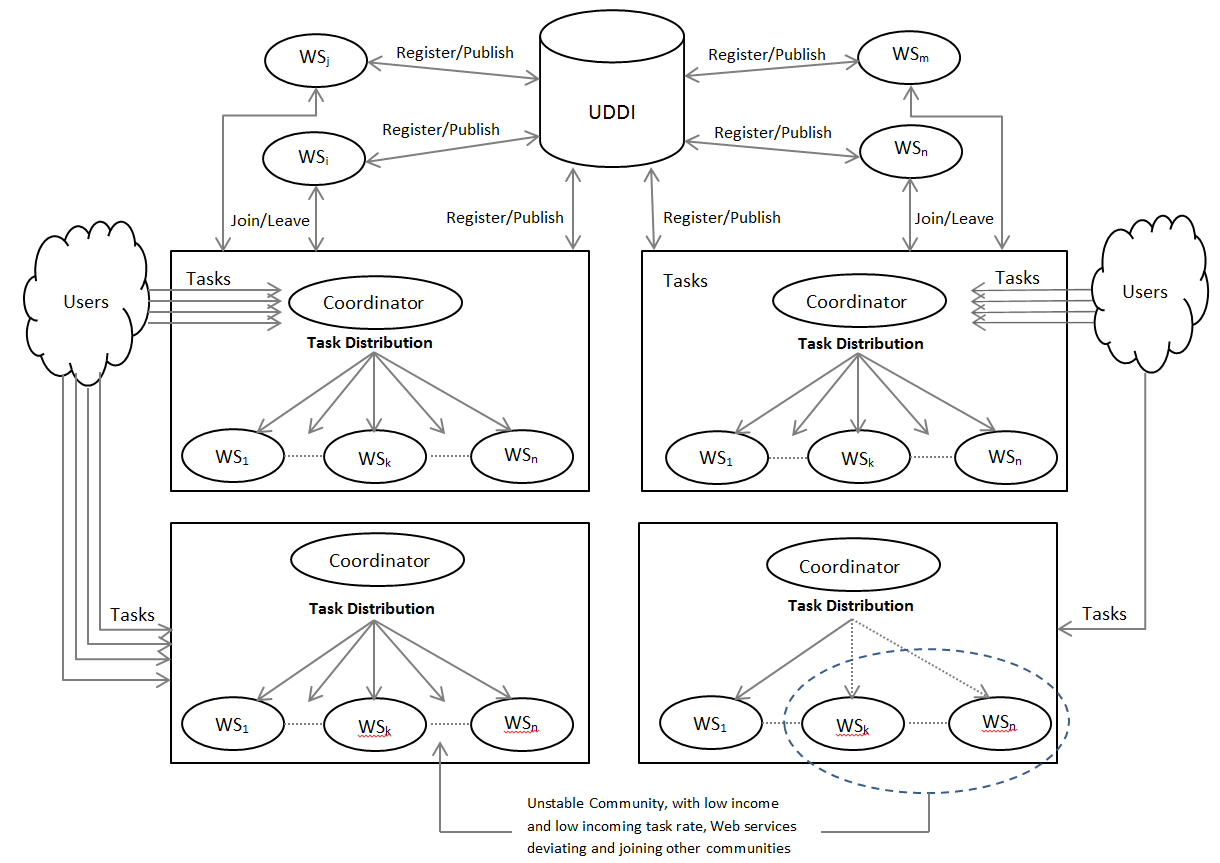
\includegraphics[width=15cm]{Figures/archss.eps}}
\caption{Architecture of Web Service communities}
\label{fig_community}
\end{figure*}


\section{Problem Formulation and Modeling}\label{s:model}

In this section, we present  web services and community coordinator's interactions, the task distribution process and revenue models in web service communities.

\subsection{Task Distribution}

As mentioned in Section \ref{webservice-communities}, communities
are robust service providers with well established market share
and reputation. By maintaining their reputation and performance,
they attract  end users which choose them as service providers to
perform their tasks. The community master is characterized by a
request rate $(R_C)$ from users. Each web service comes with a
given QoS ($QoS_{ws}$) from which the throughput $Th_{ws}$ is
excluded. Throughput is the average rate of tasks a web service
can perform per time unit. Its exclusion from $QoS_{ws}$ allows us
to build our analysis on the particular value of $Th_{ws}$. Thus,
web services perform tasks with an average output quality of
$QoS_{ws}$ and a throughput rate of $Th_{ws}$.

The community master uses a slightly modified \emph{weighted fair queuing} method to distribute tasks among its members. The goal is to allocate incoming tasks to web services with a rate matching the throughput value of $Th_{ws}$. In \emph{weighted fair queuing} method \emph{all} the input flow is multiplexed along different paths, however in our case if the input rate $(R_C)$ of the community is more than the summation of throughput values of the web services in the community, some of the input tasks will be queued and served with delay. Thus, the amount of tasks performed by community is $\sum_{ws \in C}{(Th_{ws})}$ when $\sum_{ws}{Th_{ws}} \leq R_{C}$. However, when the input rate $(R_C)$ of the community is less than the summation of throughput values of the web services in the community,
%the community has more web services having more total throughput value than community's request rate
$(R_C)$ the \emph{weighted fair queuing} algorithm assigns a weighted task rate of $R_C \times \frac{Th_{ws}}{\sum_{ws}{Th_{ws}}}$ for each web service ($ws$) and the total rate of tasks being performed is $R_C$, the community's receiving request rate.

While distributing tasks, the community master can verify the performance, throughput and quality of service of   tasks being performed by web services. It can recognize if web services are capable of doing the amount of tasks they advertised. If for any reason there is a decline in quality metrics or throughput, the  community master will announce the new parameters and community masters and members can consider those values as benchmark for future performance calculations but also to penalize them.
In this way, players have incentive to reveal their real capabilities to profit best from the community and to avoid being penalized. In addition, the system should be dynamic enough to detect and react to web services quality metrics variation as over time web service metrics may  degrade or improve, a change that the community should adjust to.
% Therefore its easy for the system to encourage players to be in some sense incentive compatible in the way that they would profit best by truthfully revealing their capabilities. Also it is important to be dynamic enough to consider web services which may have their quality metrics degraded or even improved over time for any reason and be able to adjust the community with new parameters.

\subsection{Community Revenue}

The communities and web services earn revenue by performing tasks.
The total gain is function of quality ($QoS_{ws}$) and throughput
($Th_{ws}$) of tasks being performed. As mentioned in section
\ref{ws_parameters}, $QoS_{ws}$ is obtained by a certain
aggregation function of the parameters considered in Table
\ref{qosws}. We have adopted a linear equal weight average over
all QoS parameters listed in Table \ref{qosws} excluding the
$Throughput$ and $Cost$ parameters. A community has the option to
weigh specific QoS parameters depending on the expectations of
their clients.

The maximum potential output of a community $(PO(C))$  is an aggregation of number of tasks, times their quality, for each web service member of the community:

\begin{equation}
PO(C) = \sum_{ws \in C}{(T_{ws} \times QoS_{ws})}
\end{equation}

If the summation of throughput values ($Th_{ws}$) of community members exceeds the input task rate of the community ($R_C$) the community cannot perform at its maximum potential. It denotes the case when the community has more web services than it needs to perform the input task load. The actual output has to be normalized to the amount of tasks being performed.

\begin{equation}\label{out_c}
Out(C) = \left\{
  \begin{array}{l l}
    PO(C) & \quad \text{if $\sum_{ws}{Th_{ws}} \leq R_{C}$}\\
    PO(C) \times \frac{R_{C}}{\sum_{ws}{Th_{ws}}} & \quad \text{if $\sum_{ws}{Th_{ws}} > R_{C}$}
  \end{array} \right.
\end{equation}

The revenue function of the web service community is a linear function of $Out(C)$ with a positive constant multiplier.

\subsection{Case Study}

In this section, we analyze three numerical examples and discuss the motivation of web services and community interactions and the strategies they can adopt and the revenue they can earn adopting these different strategies.


%%%%%%%%%%%%%%%%%%%%%%%%% EXAMPLE 1 %%%%%%%%%%%%%%%%%%%%%%%%%%%%%%%%%%%%
\begin{table}[!t]
\renewcommand{\arraystretch}{1.3}
% if using array.sty, it might be a good idea to tweak the value of
% \extrarowheight as needed to properly center the text within the cells
\caption{Case Study: Example 1}
\label{example_1}
\centering
\begin{tabular}{c c c c}
\hline
$WS$ & $QoS_{ws}$ & $Th_{ws}$ & $Th_{ws} \times QoS_{ws}$\\
\hline
1 & 0.8 & 4 & 3.2\\
2 & 0.8 & 5 & 4.0\\
3 & 0.8 & 3 & 2.4\\
\hline
\end{tabular}
\end{table}

\begin{table}[!t]
\renewcommand{\arraystretch}{1.3}
% if using array.sty, it might be a good idea to tweak the value of
% \extrarowheight as needed to properly center the text within the cells
% \caption{Three web services}
\label{example_1_2}
\centering
\begin{tabular}{c c || c c}
\hline
Community & Worth & Community & Worth\\
\hline
$\left\{1\right\}$ & 3.2 & $\left\{1,2\right\}$ & 7.2\\
$\left\{2\right\}$ & 4.0 & $\left\{1,3\right\}$ & 5.6\\
$\left\{3\right\}$ & 2.4 & $\left\{2,3\right\}$ & 6.4\\
$\left\{1,2,3\right\}$ & 8.0\\
\hline
Community $R_C$: 10\\
\hline
\end{tabular}
\end{table}
%%%%%%%%%%%%%%%%%%%%%%%%% EXAMPLE 1 %%%%%%%%%%%%%%%%%%%%%%%%%%%%%%%%%%%%

%%%%%%%%%%%%%%%%%%%%%%%%% EXAMPLE 2 %%%%%%%%%%%%%%%%%%%%%%%%%%%%%%%%%%%%
\begin{table}[!t]
\renewcommand{\arraystretch}{1.3}
% if using array.sty, it might be a good idea to tweak the value of
% \extrarowheight as needed to properly center the text within the cells
\caption{Case Study: Example 2}
\label{example_2}
\centering
\begin{tabular}{c c c c}
\hline
$WS$ & $QoS_{ws}$ & $Th_{ws}$ & $Th_{ws} \times QoS_{ws}$\\
\hline
1 & 0.8 & 5 & 4.0\\
2 & 0.7 & 6 & 4.2\\
3 & 0.7 & 4 & 2.8\\
\hline
\end{tabular}
\end{table}

\begin{table}[!t]
\renewcommand{\arraystretch}{1.3}
% if using array.sty, it might be a good idea to tweak the value of
% \extrarowheight as needed to properly center the text within the cells
% \caption{Three web services}
\label{example_2_2}
\centering
\begin{tabular}{c c || c c}
\hline
Community & Worth & Community & Worth\\
\hline
$\left\{1\right\}$ & 4.0 & $\left\{1,2\right\}$ & 7.4\\
$\left\{2\right\}$ & 4.2 & $\left\{1,3\right\}$ & 6.8\\
$\left\{3\right\}$ & 2.8 & $\left\{2,3\right\}$ & 7.0\\
$\left\{1,2,3\right\}$ & 7.3\\
\hline
Community $R_C$: 10\\
\hline
\end{tabular}
\end{table}
%%%%%%%%%%%%%%%%%%%%%%%%% EXAMPLE 2 %%%%%%%%%%%%%%, %%%%%%%%%%%%%%%%%%%%%%

In the first example,  we present the case of a community with
$R_C =10 $, and three web services, each having different
$QoS_{ws}$ and $Th_{ws}$ values as listed in Table
\ref{example_1}. The worth of a community is calculated based on
$Out(C)$ equation (\ref{out_c}) which is the amount of output
being generated by the community. The first table  lists the web
services with their aggregated $QoS_{ws}$ parameters, their task
input rate while working alone, and also their  throughput value
$Th_{ws}$. The second table shows all the possible communities and
their respective worth. The obtained values suggest that
communities having more web services have better gain and output.
However each community needs to  distribute the gain between web
services. Sometimes it is impossible to share the gain between all
web services in a way that no subset of them would individually
gain more if they form their own group. In this example, the value
community of ${ws_1}$ and ${ws_2}$ is 7.2, With ${ws_3}$ joining
the community the worth increases to 8.0. However there is no way
to distribute the value among web services to have  ${ws_1}$ and
${ws_2}$  earning 7.2, and ${ws_3}$ earning at least 2.4, the gain
they could earn before joining the community. This fact makes the
group unstable. In the second  example, shown in Table
\ref{example_2}, we even have situations where a web service
(${ws_3}$) joining a community ($\left\{ws_1,ws_2\right\}$)
decreases the value of community. The reason is, the community is
already full and all tasks are almost being distributed and new
community with bad quality can degrade the average quality of
tasks being done by the community. In both examples, the request
of joining of web service ${ws_3}$ should be rejected by the
community.

%%%%%%%%%%%%%%%%%%%%%%%%% EXAMPLE 3 %%%%%%%%%%%%%%%%%%%%%%%%%%%%%%%%%%%%
\begin{table}[!t]
\renewcommand{\arraystretch}{1.3}
% if using array.sty, it might be a good idea to tweak the value of
% \extrarowheight as needed to properly center the text within the cells
\caption{Case Study: Example 3}
\label{example_3}
\centering
\begin{tabular}{c c c c}
\hline
$WS$ & $QoS_{ws}$ & $Th_{ws}$ & $\text{\emph{Input Task Rate}}$\\
\hline
1 & 0.8 & 10 & 5\\
2 & 0.8 & 20 & 5\\
3 & 0.8 & 30 & 5\\
\hline
\end{tabular}
\end{table}

\begin{table}[!t]
\renewcommand{\arraystretch}{1.3}
% if using array.sty, it might be a good idea to tweak the value of
% \extrarowheight as needed to properly center the text within the cells
% \caption{Three web services}
\label{example_3_2}
\centering
\begin{tabular}{c c || c c}
\hline
Community & Worth & Community & Worth\\
\hline
$\left\{C_{ms_1}\right\}$ & 0 & $\left\{C_{ms_2}\right\}$ & 0\\
$\left\{C_{ms_1}, ws_1\right\}$ & 8 & $\left\{C_{ms_2}, ws_1\right\}$ & 8\\
$\left\{C_{ms_1}, ws_2\right\}$ & 16 & $\left\{C_{ms_2}, ws_2\right\}$ & 16\\
$\left\{C_{ms_1}, ws_3\right\}$ & 16 & $\left\{C_{ms_2}, ws_3\right\}$ & 24\\
$\left\{C_{ms_1}, ws_1, ws_2\right\}$ & 16 & $\left\{C_{ms_2}, ws_1, ws_2\right\}$ & 24\\
$\left\{C_{ms_1}, ws_1, ws_3\right\}$ & 16 & $\left\{C_{ms_2}, ws_1, ws_3\right\}$ & 32\\
$\left\{C_{ms_1}, ws_2, ws_3\right\}$ & 16 & $\left\{C_{ms_2}, ws_2, ws_3\right\}$ & 32\\
$\left\{C_{ms_1}, ws_1, ws_2, ws_3\right\}$ & 16 & $\left\{C_{ms_2}, ws_1, ws_2, ws_3\right\}$ & 32\\
$\left\{C_{ms_1}, C_{ms_2}, ...\right\}$ & 0 & $\left\{ws_1\right\}$ & 6.8\\
$\left\{ws_2\right\}$ & 4.2 & $\left\{ws_3\right\}$ & 6.8\\
\hline
Community $R_{C_1}$: 20 \\ Community $R_{C_2}$: 40\\
\hline
\end{tabular}
\end{table}
%%%%%%%%%%%%%%%%%%%%%%%%% EXAMPLE 3 %%%%%%%%%%%%%%%%%%%%%%%%%%%%%%%%%%%%

In Example 3, we consider the case of having different communities with different market share, ${R_C}$ values. Web services also have a small share of market independently, providing them with a small task pull. In these kind of scenarios, the solution considers individual maximization of payoff and also the total worth of all communities which represents the \emph{social welfare}. In this example the most efficient partition of web services is earned by having two coalitions of $\left\{C_{master_1}, ws_2\right\}$ and $\left\{C_{master_2}, ws_1, ws_3\right\}$, which yields a total value of $32 + 16 = 48$. In these types of scenarios, the goal is to reach stability, adopting a distributed approach where all players have the power of choice on the decision of whether or not they join a coalition. The communities usually start the game having some established members, encountering new web services, the communities may exchange web services and new web services would join them having at least one player gaining utility, without hurting any other participant. In this example if we initially having two coalitions of $\left\{C_{master_1}, ws_2\right\}$ and $\left\{C_{master_2}, ws_1\right\}$ and a ${ws_3}$ as new web service, ${ws_3}$ joining ${C_{master_1}}$ would hurt at least itself or $ws_2$, however ${ws_3}$ joining ${C_{master_2}}$ would not hurt any participants and ${ws_3}$ would earn more within the community and the community will have enough web services performing the incoming tasks from users.

The first two examples illustrate the fact that a community cannot simply increase its revenue by adding more web services. The web services and even community owners are autonomous agents and would deviate and be displeased about the community if new members cause a drop in their profit. The job of the community master is to attract as many quality web services it can and keep them satisfied; hence the group stability is guaranteed.
The third example highlights another type of problem we would like to address, which is how to form best possible groups of communities, and allocate web services among communities in a way which would maximize payoff for of our agents and members already residing in the communities.
In next section, we provide collaborative game theory based algorithms for our autonomous agents, to tackle these problems and find applicable and efficient strategies for communities and web services to maximize their profit.

 \section{Web Service Cooperative Games}\label{s:game_solution}

In this section, we present different web service community models
and focus on the problem of how both web services and community
masters as rational entities would adopt strategies to maximize
their payoff.

\subsection {Web Services and One Community}

In this scenario, we assume the existence of a typical community
managed by its master, and web services need to join it to be able
to get requests from the master. The community master is
characterized by a requests rate $(R_{C})$ from users. Each web
service comes with a given QoS ($QoS_{ws}$). The worth of a community
$v(C)$ is set to Out(C) based on equation \ref{out_c}.

As mentioned in previous section, the worth and output of a
community  is a function of the
throughput and provided QoS of its web service members. If the throughput rate is more than
the master's input request rate, it means the web services inside
the community are capable of serving more requests than the
demand. Considering this factor, the valuation function is
designed to balance the output performance so that it matches the
exact throughput rate and QoS the web service can provide within
the particular community.
%** In the case where the limited tasks are distributed among web services uniformly, the value of coalition would be the proportion of the average QoS times their throughput to rate of available requests. **

In this first scenario, we only consider one grand coalition and
analyze the system from the point of view of one single master web
service and a collection of web services. The master web service
decides which members can join
%or should leave%
the community and distributes the requests and income among its
community members (see Figure \ref{fig_sim1}).

\begin{figure}[!t]
\centering
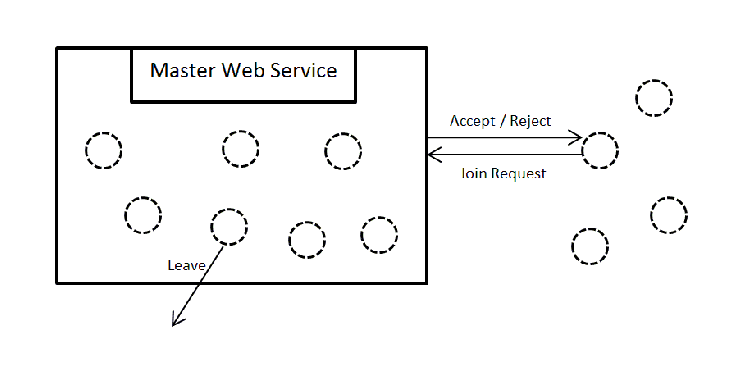
\includegraphics[width=3in]{Figures/s1.eps}`
\caption{Web Services and A Grand Community}
\label{fig_sim1}
\end{figure}

The membership decision is made based on throughput and \emph{QoS}
of the considered web service. The goal is to have quality web
services in the community so it stays stable and no other web
services would have incentives to deviate and leave the coalition
$C$. Therefore, a basic method would be to check the core of the
coalition $C$ considering all the current community members (all
web services already residing within the community) and the new
web service. This algorithm uses the \emph{Shapley value}
distribution method as described in Equation \ref{eq:shapley} to
distribute the gain of $v(C)$ among all the members and then
checks if the \emph{Shapley value} payoff vector for this
community having the characteristic function $v(C)$ is in the
\emph{core}. In the \emph{Shapley value} payoff vector, the payoff
for each web service $ws_i$ is calculated based on its marginal
contribution $v(C \cup {i}) - v(C)$ over all the possible
different permutations in which the coalition can be formed, which
makes the payoff distribution fair. Because of going through all
the possible permutations of subsets of $N$, the nature of the
\emph{Shapley value} is combinatorial, which makes it impractical
to use as the size of our coalitions grows. However, it is proven
that in convex games, the \emph{Shapley value} lies in the core
\cite{DBLP:conf/ijcai/GrecoMPS11, myerson1991game}. Thus, if the
\emph{Core} is non-empty, the payoff vector is a member of the
\emph{Core}. The following proposition is important to make our
algorithm tractable.
% so in our algorithm we check the core membership of this payoff vector.

%\ref{eq:convex}.

%\newtheorem{theorem}{Proposition}
%\begin{theorem}[Einstein-Podolsky-Rosenberg]
\begin{theorem}\label{proposition1}
A game with a characteristic function $v$
is convex if and only if for all $S$, $T$, and $i$ where $S
\subseteq T \subseteq N \backslash \left\{i\right\}, \forall i \in
N$,
%For $\forall S \subseteq T \subseteq N \backslash \left\{i\right\}, \forall i \in N$ we have:
\begin{equation}\label{eq:convex_snow}
v(S \cup \left\{i\right\}) - v(S) \leq v (T \cup \left\{i\right\}) - v(T)
\end{equation}
\end{theorem}

%\begin{Proposition}\label{proposition} A game with a characteristic function $v$
%is convex if and only if for all $S$, $T$, and $i$ where $S
%\subseteq T \subseteq N \backslash \left\{i\right\}, \forall i \in
%N$,
%For $\forall S \subseteq T \subseteq N \backslash \left\{i\right\}, \forall i \in N$ we have:
%\begin{equation}\label{eq:convex_snow}
%v(S \cup \left\{i\right\}) - v(S) \leq v (T \cup \left\{i\right\}) - v(T)
%\end{equation}
%\end{Proposition}

\begin{proof}
We first prove the ``only if'' direction:
%\\$~~~~$\textbf{1}. ``only if'' direction:\\
\\$~~~~$\ \textbf{1}. ``only if'' direction:\\
%\setlength{\abovedisplayshortskip}{2pt}
Assume:\\
\vspace{-0.5cm}
\begin{gather*}\label{convexsnowproof}
v(S \cup \left\{i\right\}) - v(S) \leq v (T \cup \left\{i\right\})
- v(T)
\\
\rightarrow v(S \cup \left\{i\right\}) + v(T) \leq v (T \cup \left\{i\right\}) + v(S)
\end{gather*}

Considering $S \subseteq T$:
\setlength{\abovedisplayshortskip}{2pt}
\begin{gather*}
T \cup \left\{i\right\} = (S \cup \left\{i\right\}) \cup T
\\
S = (S \cup \left\{i\right\}) \cap T
\end{gather*}

By setting $A = S \cup \left\{i\right\}$ and $B = T$ we have:
\setlength{\abovedisplayshortskip}{2pt}
\begin{gather*}
v(S \cup \left\{i\right\}) + v(T) \leq v (T \cup \left\{i\right\}) + v(S)
\\
\rightarrow v(S \cup \left\{i\right\}) + v(T) \leq
\\
v((S \cup \left\{i\right\}) \cup T) + v((S \cup \left\{i\right\}) \cap T)
\\
\rightarrow v(A) + v(B) \leq v(A \cup B) + v(A \cap B)
\end{gather*}
Consequently, the game is convex.

\textbf{2}. ``if'' direction:\\
Assume the game is convex. Thus, for all $A, B \subset N$, we
have: \setlength{\abovedisplayshortskip}{2pt}
\begin{gather*}
v(A) - v(A \cap B) \leq v(A \cup B) - v(B)
\end{gather*}

By setting $S \cup \left\{i\right\} = A$ and $T = B$ where $S \subseteq T$:
\setlength{\abovedisplayshortskip}{2pt}
\begin{gather*}
v(S \cup \left\{i\right\}) - v((S \cup \left\{i\right\}) \cap T) \leq v(T \cup (S \cup \left\{i\right\})) - v(T)
\\
\rightarrow v(S \cup \left\{i\right\}) - v(S) \leq v(T \cup \left\{i\right\}) - v(T)
\end{gather*}

\end{proof}

Thus, in order to keep the characteristic function convex, new web
services should have more marginal contribution as the coalition
size grows.

Our algorithm works as follows. Given an  established community
with a master and some member web services, a web service would send a \emph{join request} to join  the
community. Ideally, the \emph{core}
or \emph{$\epsilon$-core} stability of the group having this new
member should be analyzed. As the normal core membership algorithm is computationally
intractable, we exploit Proposition \ref{proposition1} and Equation
\ref{eq:convex_snow} to check the convexity of our game having
characteristic function where the new member is added. In the
equation, let $C$  be our community members before
having the new web service join the community. Let  ${i}$ be the new web
service, and then verify the equation for $S$, setting $ S = T /
W1 $ where $W1$ is the set of all possible subsets of the set $N$
having the size $1$. We can relax the equation a bit by adding a
constant $\epsilon$ to the left side of the equation. We call this
method \emph{Depth-1 Convex-Checker} algorithm. If the equation is
satisfied for all $W1$, we let the new web service join our
community, since the web service will contribute positively enough
to make our new community stable. Since only subsets of size $1$
are checked, the following Proposition holds.

\begin{theorem}\label{complexity1}
\emph{The run time complexity of Depth-1 Convex-Checker algorithm is
$O(n)$.}
\end{theorem}

By this result, we obtain a significant reduction from $O(2^n)$,
which is the complexity of checking all possible subsets of $N$.
In our second method, we use the same algorithm, but this time we
set $W2$ to be the set of all possible subsets of size two and one
of the community $C$. We call this method \emph{Depth-2
Convex-Checker} and its run time complexity is still
linear:

\begin{theorem}\label{complexity2}
\emph{The run time complexity of Depth-2 Convex-Checker algorithm is
$O(n^2)$.}
\end{theorem}

It is possible to develop an algorithm that continues the
verification of this condition against subsets of size $3$,
$4$, etc. until the algorithm gets interrupted.

\subsection {Web Services and Many Communities}

In this scenario, we consider multiple communities managed by
multiple master web services, each of which is providing
independent request pools (see Figure \ref{fig_sim2}). Identical
to the first scenario, master web services form coalitions with
web services. We use coalition structure formation methods to
partition web services into non-empty disjoint coalition
structures. As mentioned in Section \ref{sec:coalition}, the used
algorithms in \cite{Sandholm:1999:CSG:317145.317152,DBLP:conf/ijcai/GrecoMPS11,DBLP:conf/ijcai/RahwanMJ11} try to
solve key fundamental problems of what coalitions to form, and how
to divide the payoffs among the collaborators.

\begin{figure}[!t]
\centering
\includegraphics[width=3in]{Figures/s2.eps}
\caption{Web Services and Many Communities}
\label{fig_sim2}
\end{figure}

In coalition-formation games, formation of the coalitions is the
most important aspect. The solutions focus on maximizing the
social welfare. For any coalition structure $\pi$, let
$v_{cs}(\pi)$ denote the total worth $\sum_{C \in \pi}{v(C)}$,
which represents the \emph{social welfare}. The solution concepts
in this area deal with finding the maximum value for the social
welfare over all the possible coalition structures $\pi$. There
are $centralized$ algorithms for this end, but these approaches
are generally NP-complete. The reason is that the number of all
possible partitions of the set $N$ grows exponentially with the
number of players in $N$, and the centralized algorithms need to
iterate through all these partitions.
%These algorithms \cite{DBLP:conf/ijcai/GrecoMPS11, DBLP:conf/ijcai/RahwanMJ11, RePEc:wpa:wuwpga:0110001} are centralized algorithms, where all the complexity. However these algorithms are more intractable than Core stable solutions and practical with some constraints in practice\cite{RePEc:wpa:wuwpga:0110001}.
In our model, we propose using a distributed algorithm where each
community master and web service can be a decision maker and
decide for its own good. The aim is to find less complex and
distributed algorithms for forming web services coalitions
\cite{DBLP:journals/igtr/AptW09,Dieckmann02dynamiccoalition,ray2007game}.
The distributed merge-and-split algorithm in
\cite{DBLP:journals/igtr/AptW09} suits our application very well.
It keeps splitting and merging coalitions to partitions which are
preferred by all the players inside those coalitions.

This merge-and-split algorithm is designed to be adaptable to
different applications. One major ingredient to use such an
algorithm is a preference relation or well-defined orders proper
for comparing collections of different coalition partitions of the
same set of players. Having two partition sets of players, namely
$P = {P_1,...,P_k}$ and $Q = {Q_1,...Q_l}$, one example would be
to use the social welfare comparison $\sum^k_{i=1}v(P_i) >
\sum^l_{j=1}v(Q_j)$. For our scenario, we use \emph{Pareto order}
comparison, which is an individual-value order appropriate for our
self-interest web services. In the Pareto order, an allocation or
partition $P$ is preferred over another $Q$ if at least one player
improves its payoff in the new allocation and all the other
players still maintain their payoff ($p_i \geq q_i$ with at least
one element $p_i > q_i$).

The valuation function $v(C)$ for this scenario is the same as
\emph{``Web Services and One Community''} scenario. However, in
order to prevent master web services joining the same community,
we set $v(C) = 0$ when $C$ has either none, or more than one
master web service as member.

In this scenario, as new web services are discovered and get ready
to join communities, our algorithm keeps merging and splitting
partitions based on the preference function. The decision to merge
or split is based on the fact that all players must benefit. The
new web services will merge with communities if $all$ the players
are able to improve their individual payoff, and some web services
may split from old communities, if splitting does not decrease the
payoff of \emph{any} web service of the community. According to
\cite{DBLP:journals/corr/abs-cs-0605132}, this sequence of merging
and splitting will converge to a final partition, where web
services cannot improve their payoff. More details of this
algorithm and analysis of generic solutions on coalition formation
games are described in \cite{DBLP:journals/igtr/AptW09}.

\subsection{Taxation, Subsiding and Community Stability}\label{s:tax}

ssed $core$ as one of the prominent solution concepts in cooperative games. Working together, completing tasks and generating revenue, agents need to distribute the gain in a way no agents would gain more by having their own group. However, in most cases the core of a game is empty so we introduced the \emph{$\epsilon$-core} concept, where agents would only earn a minimal amount of $\epsilon$ by deviating. Stability is an attractive property for communities. In addition, communities would benefit by having slightly more web services then the exact number of web services satisfying task rate cap. This is because  there is always a possibility that the agents may leave the community or they may under perform and degrade the quality values they were initially performing with.

One way for communities to ensure  stability could be  by applying a tax, $\epsilon$ amount of cost for web services changing communities which would make deviation a costly act. However this would require all community coordinators to agree on a same amount of taxation, being governed by some external entities or web services would join communities with lesser amount of tax. Another viable solution to our scenario is to stabilize the game using external subsidies. The reason a gamWe discue is not stable is that the community is not making enough revenue to allocate  enough gain to the players. A community master can subside its community with a constant coefficient value of $\lambda$.

Rewarding a community with high number of quality participants with $\lambda v(C)$, where $\lambda \leq 1$.

Obviously with a big number of $\lambda$, it is always possible to stabilize the community. However, this can be a costly act for community masters so they are interested in the minimum subside value of $\lambda$ making the game stable. Subsiding or taxing in order to reduce the bargaining power of sub coalitions are called $taxation$ \cite{eps346856} methods.



%Thus, another way to garantee \emph{$\epsilon$-core} stability can be achieved by some surplus payments from community coordinators. These concepts of applying cost in coallition values in order to reduce their bargaining power are called $taxtation$ methods\cite{eps346856}.

%The \emph{$\epsilon$-core} concept, in its definition, considers the willing to join or deviate from agent's point of view. It claims agents for any reason will be not willing to deviate to gain less than $\epsilon$ amount of profit. Communities can agree on However, in our case, the community master is willing to keep web services in communities too. There are several reasons for this, one reason is there is always possibility that agents may leave the community or they may under perform from the quality values they were initially performing with. To this end, our communities will reward and valuate web services in the community



\section{Experimental Results and Analysis}\label{s:resutls}

In this section, we discuss the experiments we performed for our
scenarios to validate the applicability and performance of our
proposed methods in realistic environments. We created a pool of
web services and populated most of their \emph{QoS} parameters
from a real world web service dataset
\cite{DBLP:conf/smc/Al-MasriM09a}. We implemented the simulations
using Java and executed the simulations on an Intel Xeon X3450
machine with 6GBs of memory. For other parameters missing from the
dataset, we used normal random distribution with parameters
estimated using the method of maximum likelihood.

One of the key criteria reflecting the performance of web service
coalitions is the user satisfaction. User satisfaction can be
measured in terms of quality and quantity of requests (or tasks)
successfully answered by the communities. We initiated the
communities with few web services, then let rejecting and
accepting random web services go for a short number of iterations.
After that, we started the request distribution for the communities
and let them allocate requests among member web services.
Thereafter, we measured the average output performance of tasks in
communities following different methods.

\begin{figure}[!t]
\centering
%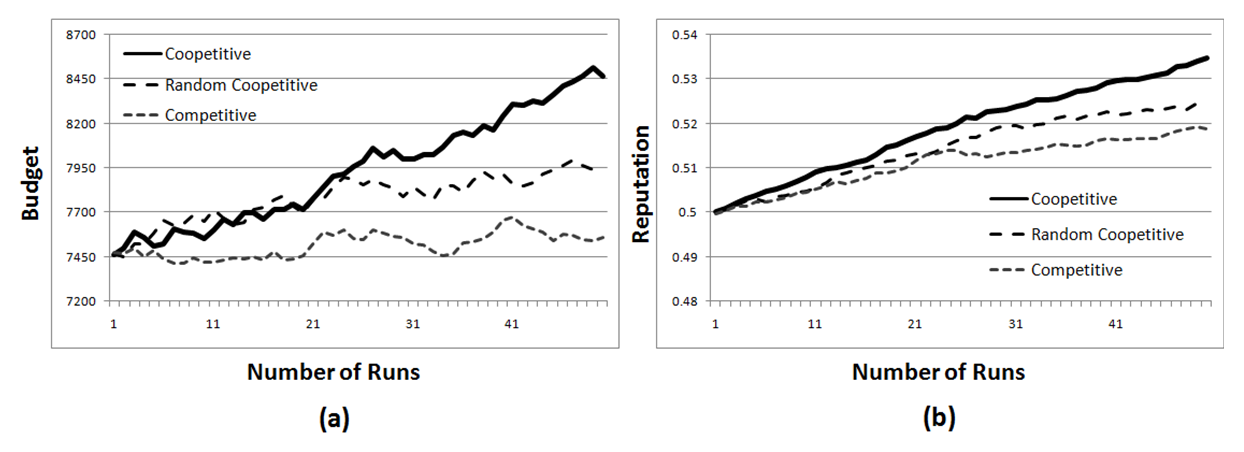
\includegraphics[scale=0.6]{graph1Final+.eps}
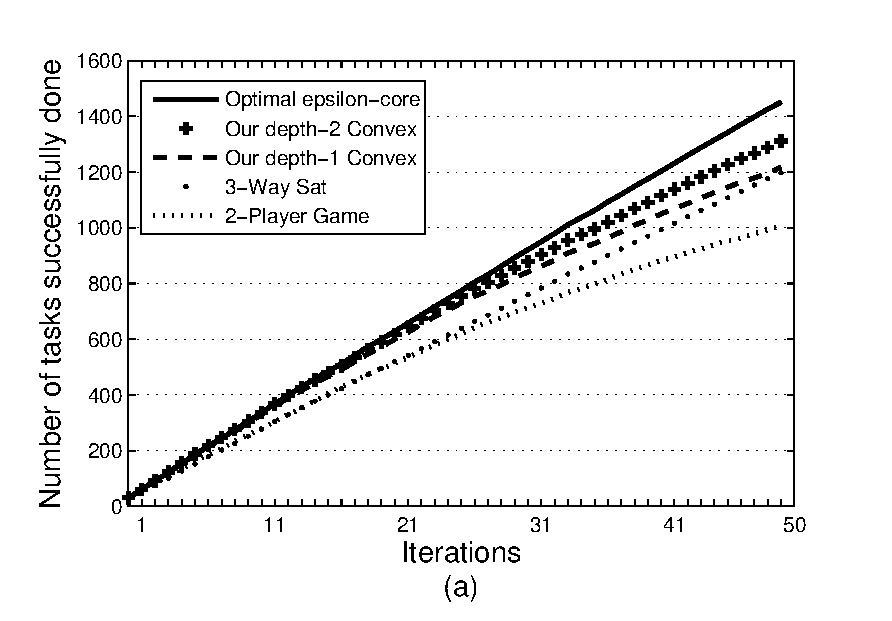
\includegraphics[width=3in]{Figures/task_done_opt.eps}
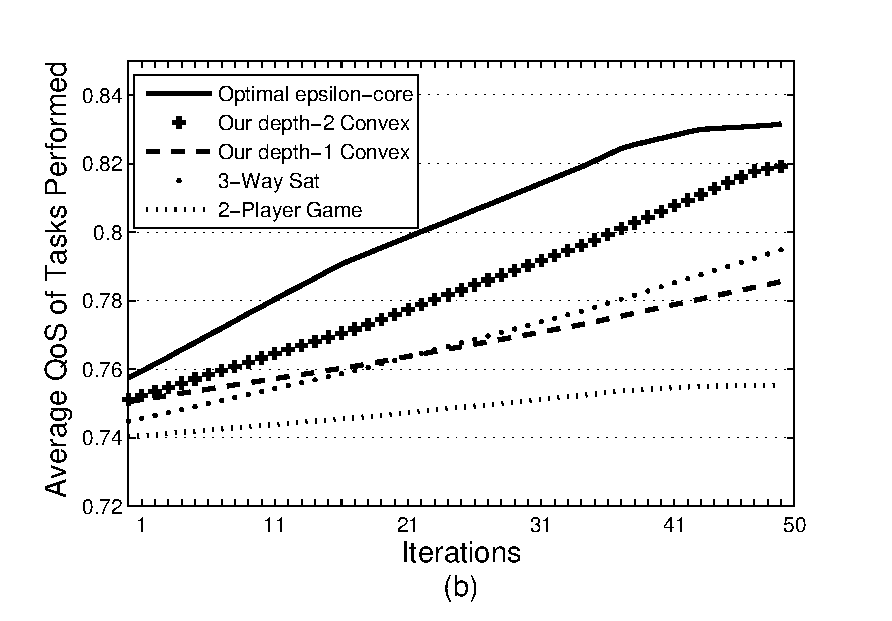
\includegraphics[width=3in]{Figures/task_qos_opt.eps}
\caption{Part (a): Cumulative number of requests successfully
done. Part (b): Average QoS of requests performed.}
\label{performanceall}
\end{figure}

Figure \ref{performanceall} depicts the results of optimal
\emph{$\epsilon$-core}, \emph{Depth-1 Convex-Checker},
\emph{Depth-2 Convex-Checker}, \emph{3-Way Satisfaction}
\cite{DBLP:conf/IEEEscc/LimTMB12}, and \emph{2 Player
Non-Cooperative} \cite{DBLP:conf/IEEEscc/KhosravifarABT11} methods
in \emph{one grand community with many web services} scenario.

For the \emph{optimal core} method we have used the well known \emph{$\epsilon$-core} method as the
taxtation method to relax the core condition to help communities, attract web services.
We have assigned $\epsilon$ to 15\% of total community worth, $\epsilon = 0.15 \times v(C)$, which allows
subsets of the coalition to gain maximum 15\% of $v(C)$. In the
\emph{optimal $\epsilon$-core} method, we capped the coalition
size to 25 web services, since the method is computationally
intractable as number of web services increase and anything more than that would make it
impractical to run in our simulations. In the other methods, there
were no cap on size of the community and we had communities of
size 60 web services at some points. In this scenario our community receives 30 tasks on average per iteration, from users. The community, after the task distribution process on each iteration, will reevaluate QoS metrics of its members and can check for new membership requests. Web services may join or leave the community between iterations. The results show that our
\emph{depth-2 convex checker} method is performing better compared
to the other methods and its performance is close to optimal
\emph{$\epsilon$-core} method. Our \emph{depth-1 convex checker}
and the \emph{3-Way Satisfaction} method, are also performing well.

\begin{figure}[!t]
\centering
%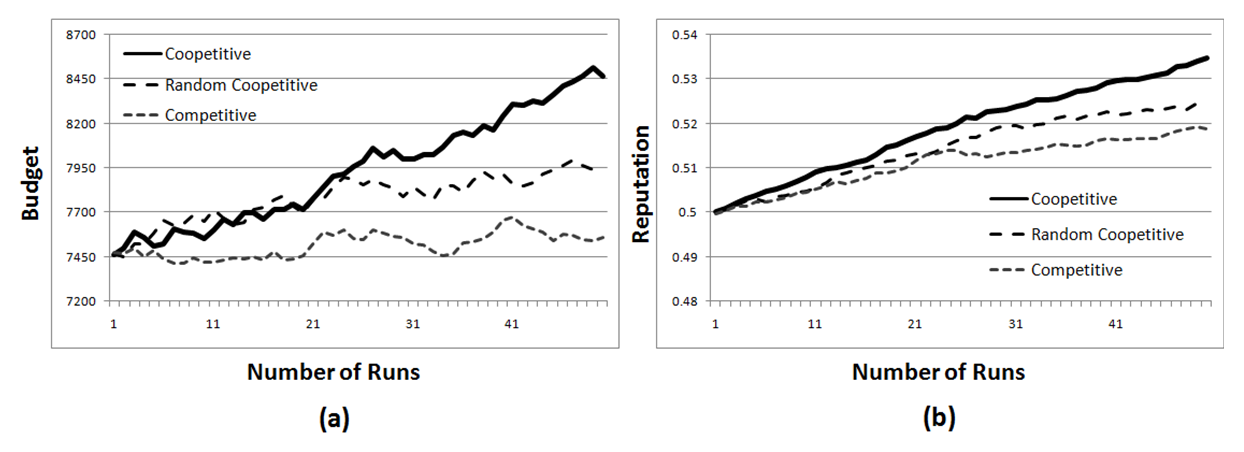
\includegraphics[scale=0.6]{graph1Final+.eps}
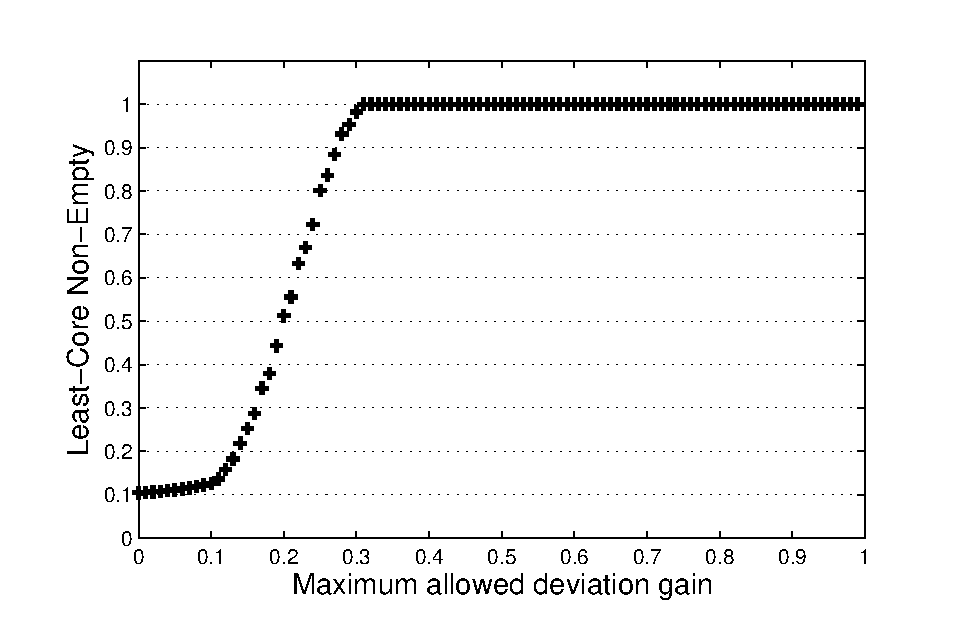
\includegraphics[width=3in]{Figures/least_core.eps}
\caption{Analysis of \emph{$\epsilon$-core} set non-emptiness, for different values of $\epsilon$} \label{f_leastcore}
\end{figure}

As mentioned in Section \ref{s:preliminaries}, the concept of
\emph{core}, assumes no coalition of players can gain anything by
deviating, which is a fairly strong requirement, and that is why
the notion of \emph{$\epsilon$-core} was introduced. Least-Core
$e(G)$ of a game $G$, is the minimum amount of $\epsilon$ so that
the core is not empty. We evaluated the non-emptiness of \emph{$\epsilon$-core} set using the
valuation function and a set of web services. We picked random
number of web services from the dataset and formed around 10,000
random coalitions consisting of 3 to 26 web services. We choose 26
as the maximum number of members in our coalition since it
is computationally very complex for larger coalitions to verify whether
\emph{$\epsilon$-core} set is empty or not. Also instead of considering $\epsilon$ amount of constant deviation in \emph{$\epsilon$-core} definition (Equation \ref{eq:core2}), we similarly defined \emph{relative $\epsilon$-core} concept where no coalition would benefit more than \emph{$\epsilon$ $\times$ v(C)} by deviating. We set $\epsilon$ between 0 and 1 and verify the \emph{relative $\epsilon$-core} set non-emptiness. The results in Figure
\ref{f_leastcore} illustrates that almost 10\% of our random web
service coalitions have non-empty \emph{core} solution and
\emph{$\epsilon$-core} solution is \emph{always} non-empty when we
let agents gain only 30\% more of $v(C)$ by deviating.

One of the properties of coalition structure formation algorithms
in our second scenario is that they partition web services with low
throughput rate so that they usually join coalitions with less
request rate. Since the characteristic function $v(C)$ and the
fair Shapely payoff vector is proportional to web services'
contribution, the web services with small contribution will get
paid much less in communities having web services with high
throughput. On the other hand, according to the valuation function
$v(C)$, web services with high throughput will not contribute well
to communities with low amount of user requests (low market
share). The strong web services are likely to deviate from weak
coalitions, joining a stronger one, which makes the initial
coalition unstable.


\begin{figure}[!t]
\centering
%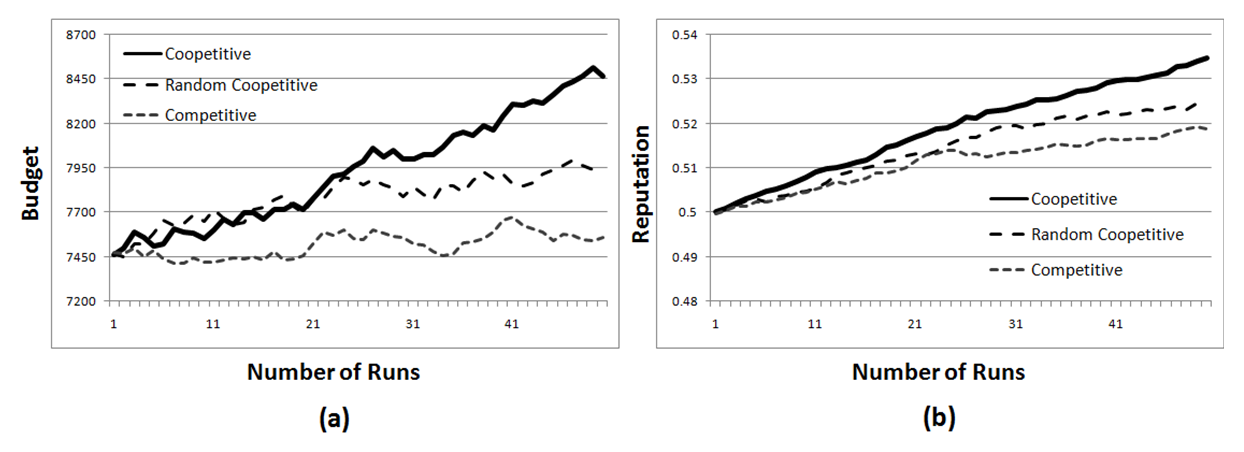
\includegraphics[scale=0.6]{graph1Final+.eps}
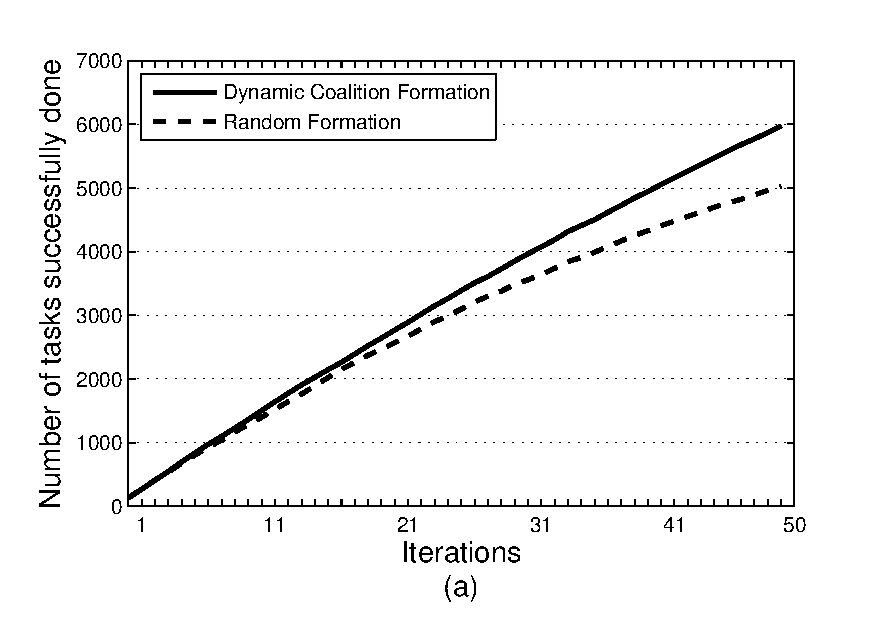
\includegraphics[width=3in]{Figures/s2_task_done.eps}
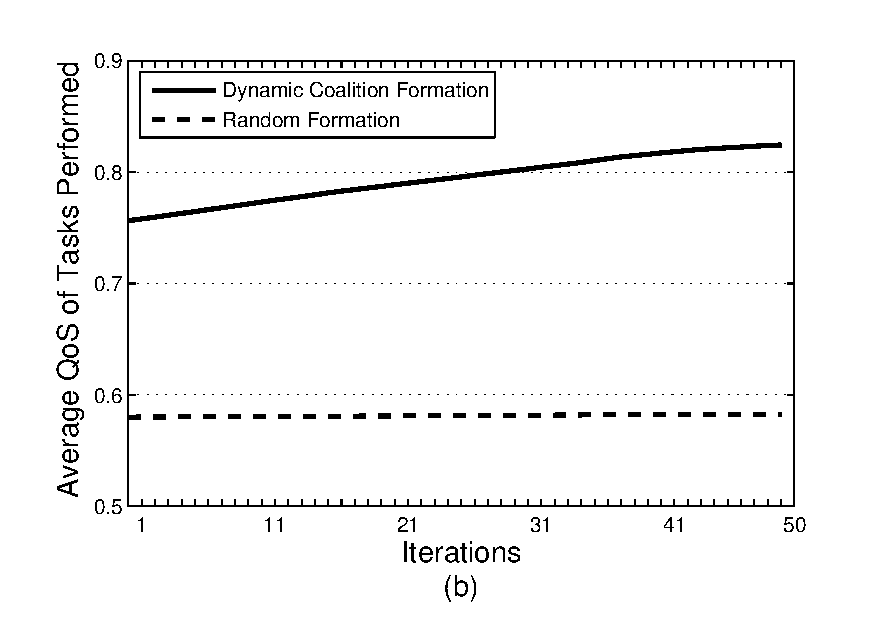
\includegraphics[width=3in]{Figures/s2_task_qos.eps}
\caption{Part (a): Cumulative number of tasks succesfully done. Part
(b): Average QoS of tasks performed.} \label{performancemany}
\end{figure}

In Figure \ref{performancemany}, we compare our \emph{Web Services
and many Communities} scenario with a method which ignores QoS
parameters and forms coalitions by allowing web services to join
only if they have enough requests for themselves. In other words,
web services can join a community when the request rate is less
than the throughput of all the member web services. We name this
method \emph{Random Formation} and use it as a benchmark for our
QoS-aware coalition formation process. In this scenario, each user individually generates randomly
between 0 to 10 number of tasks per iteration, then the users target a community and direct their requests to the chosen community. As the results illustrate,
our method forms better coalitions of web services improving
performance and satisfaction for both web services and coalitions.

\begin{figure}[!t]
\centering
%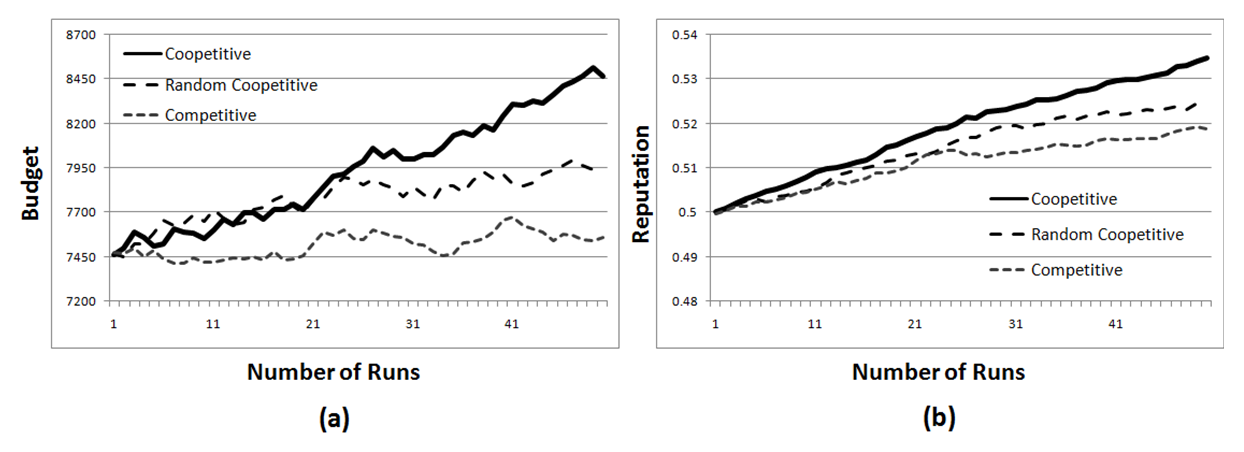
\includegraphics[scale=0.6]{graph1Final+.eps}
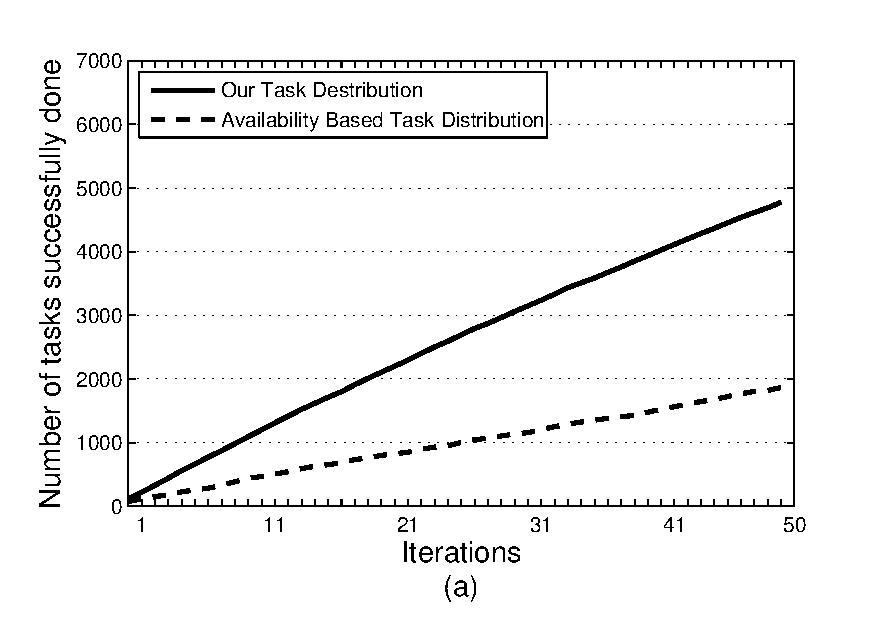
\includegraphics[width=2.5in]{Figures/avg_task_ws_done.eps}
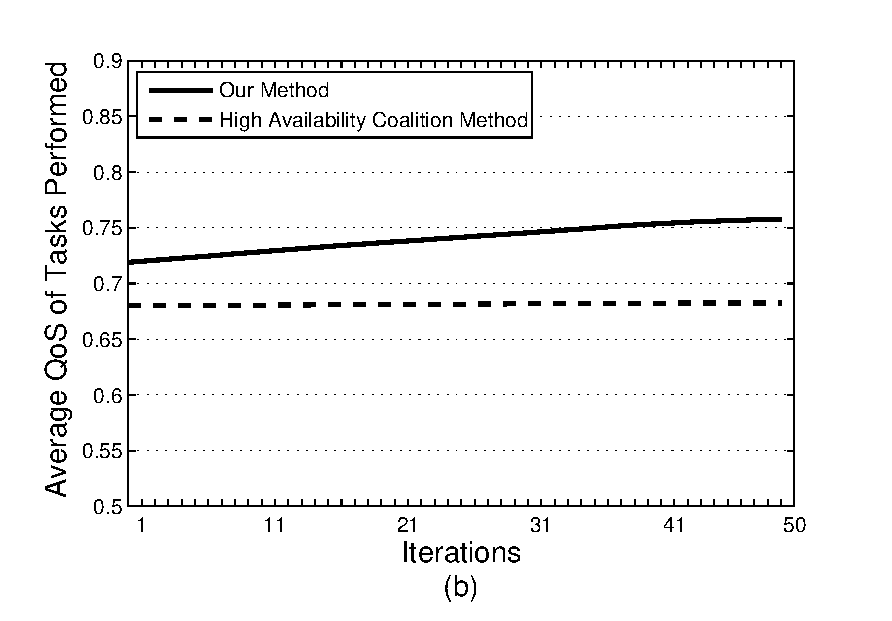
\includegraphics[width=2.5in]{Figures/avg_qos_ws_done.eps}
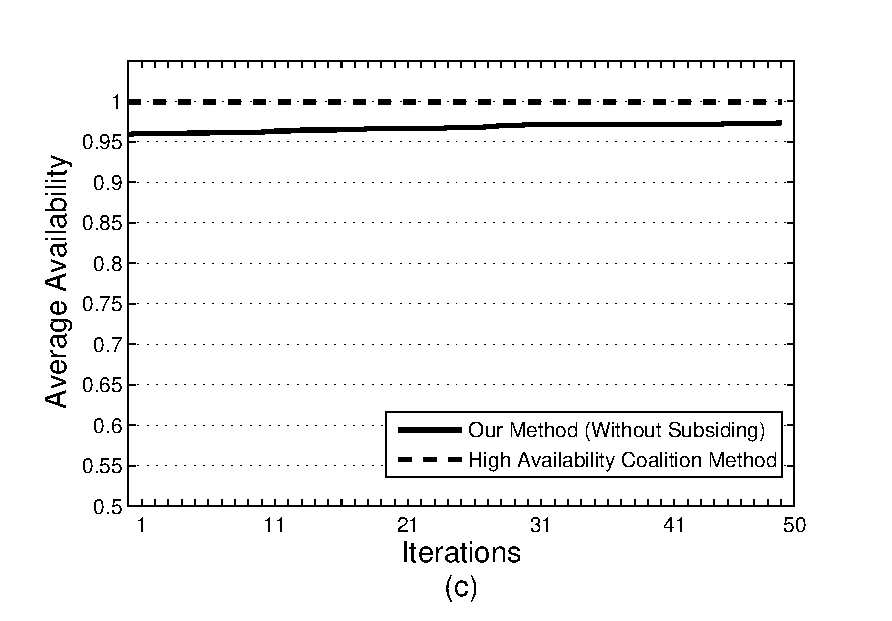
\includegraphics[width=2.5in]{Figures/avg_avail_ws_done.eps}
\caption{A comparison between our community model and the high availability community model, on communities of size 4,5,6 only. Part (a): Cumulative number of tasks succesfully done. Part
(b): Average QoS of tasks performed. (c) Average Community Service Availability} \label{fig_avail_method}
\end{figure}

Finally, in our last experiment, we compare our work with the work
in \cite{10.1109/TSC.2012.12} which we call it \emph{High
Availability Coalition} method, because of nature of their
community valuation function, which focuses on community
availability as main consideration. Their community formation
model is very different than ours, however we have been very
careful to make the experiment environment as fair and similar as
possible. We limited our maximum community size by 5 in order to
have communities with almost the same size. In their method, they
have used web services as backups rather than active collaborative
players, and they only get task when the first web service in an
ordered chain fails to perform the task. However with recent
advancement in cloud and hardware infrastructures availability is
less of an issue for web services, and web services are highly
available. Part(a) of figure \ref{fig_avail_method} shows our
method performs almost performs tasks successfully with rate of
three times more than \emph{High Availability Coalition} method
because of real cooperative nature and task distribution of our
algorithm. This result shows using web services as backups, and
not as real collabrative players is a huge waste of web service
capability since they have very low chance of getting jobs and its
the primary web service (the first in their coordination chain)
which does most of the work. The average quality of service of
tasks performed is also better since our method considers all
quality of service metrics mentioned in Table \ref{qosws}. Part(c)
shows the availability of community from end user point of view.
The \emph {High Availability Coalition} method almost has 100\%
uptime since they use web services as backups, so the chance of
job failing reduces significantly as community members increase.
In our method we have more chance of fail for each web service,
however with some subsiding, and hiring a few more web service
they can compensate the low chance of failure of web services in
our community.
